% sezione intro frame 00
\begin{frame}
    \frametitle{Git intro}
    \framesubtitle{Getting started with Git}
    \addtocounter{nframe}{1}
    
    \begin{block}{VCS}
        Version control (VCS) is a system that records changes to a file or set of files over time so that you can recall specific versions later.
    \end{block}

\end{frame}

\begin{frame}
    \frametitle{Git intro}
    \framesubtitle{Getting started with Git}
    \addtocounter{nframe}{1}

    \begin{block}{Benefits}
        \begin{itemize}
            \item It allows you to revert selected files back to a previous state
            \item compare changes over time
            \item who last modified something that might be causing a problem
            \item \dots
        \end{itemize}
    \end{block}

\end{frame}


% sezione intro frame 01
\begin{frame}
    \frametitle{Git and GitHub}
    \framesubtitle{Getting started with Git}
    \addtocounter{nframe}{1}
    
    \begin{block}{VCS Main feature}
        Using a VCS also generally means that if you screw things up or lose files, you can easily recover
    \end{block}

\end{frame}

% sezione intro frame 01
\begin{frame}
    \frametitle{Git and GitHub}
    \framesubtitle{Getting started with Git}
    \addtocounter{nframe}{1}
    
    \begin{block}{Different VCS Architectures}
        \begin{itemize}
            \item Local Version Control System (RCS)
            \item Centralized Version Control System (CVS, SVN)
            \item Distributed Version Control System (GIT, Mercurial)
        \end{itemize}
    \end{block}

\end{frame}

% sezione intro frame 01
\begin{frame}
    \frametitle{Git and GitHub}
    \framesubtitle{Getting started with Git}
    \addtocounter{nframe}{1}
    
    \begin{block}{Local Version Control System}
        \begin{center}

            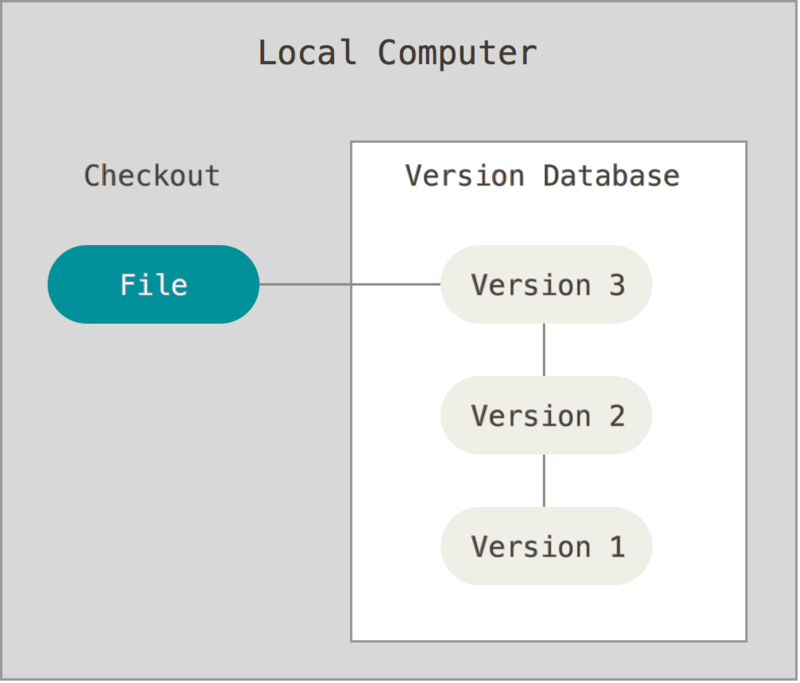
\includegraphics[width=.55\textwidth]{imgs/local.png}
    
        \end{center}
    
    \end{block}

    \textit{database that kept all the changes to files under control}

\end{frame}

% sezione intro frame 01
\begin{frame}
    \frametitle{Git and GitHub}
    \framesubtitle{Getting started with Git}
    \addtocounter{nframe}{1}
    
    \begin{block}{Centralized Version Control System}
        \begin{center}

            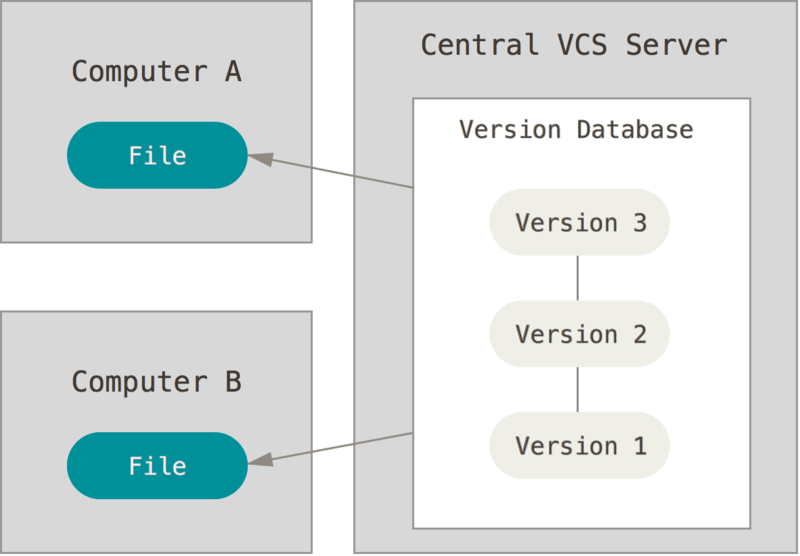
\includegraphics[width=.6\textwidth]{imgs/centralized.png}
    
        \end{center}
    
    \end{block}

    \textit{Need to collaborate: single server that contains all the files}

\end{frame}


% sezione intro frame 01
\begin{frame}
    \frametitle{Git and GitHub}
    \framesubtitle{Getting started with Git}
    \addtocounter{nframe}{1}
    
        \begin{center}

            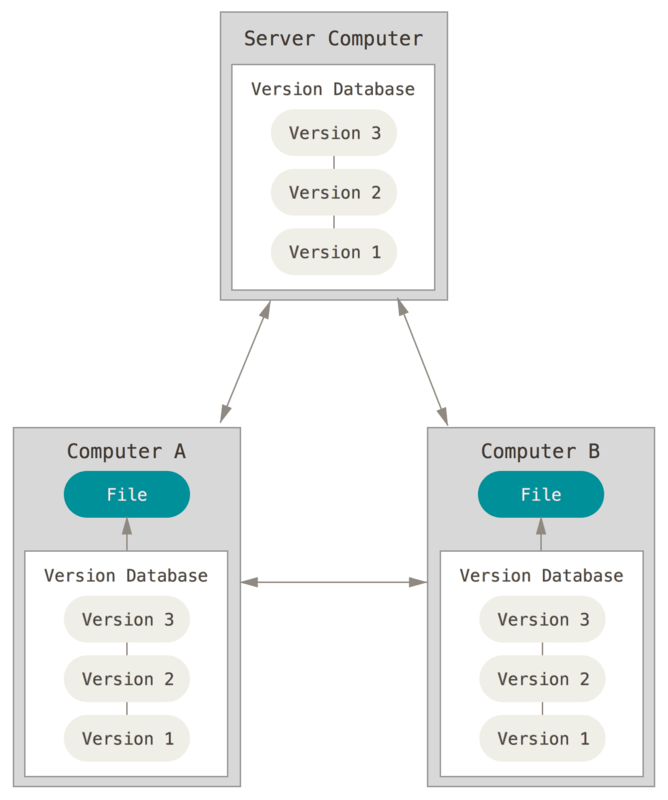
\includegraphics[width=.5\textwidth]{imgs/distributed.png}
    
        \end{center}
    
    \textit{Client repositories can be copied back up to the server to restore it}

\end{frame}

\begin{frame}
    \frametitle{Git and GitHub}
    \framesubtitle{Getting started with Git}
    \addtocounter{nframe}{1}
    
    \begin{block}{GIT DVCS}
       \begin{itemize}
           \item Started by Linux community
           \item Fast and efficient 
           \item Simple design
           \item non-linear development
           \item fully distributed
           \item handle large projects
           \item easy to use
       \end{itemize}
    
    \end{block}

\end{frame}

\begin{frame}
    \frametitle{Git and GitHub}
    \framesubtitle{Getting started with Git}
    \addtocounter{nframe}{1}
    
    \begin{block}{GIT DVCS}
        With Git, every time you commit, or save the state of your project, Git basically \textbf{takes a picture of what all your files look like} at that moment and stores a \textbf{reference to that snapshot}.    
    \end{block}

\end{frame}

\begin{frame}
    \frametitle{Git and GitHub}
    \framesubtitle{Getting started with Git}
    \addtocounter{nframe}{1}
    
    \begin{block}{GIT DVCS}
        Everything in git is \textbf{checksummed before it is stored} and is then referred to by that checksum
    \end{block}

    \begin{block}{GIT DVCS}
        40-character string composed of hexadecimal characters
    \end{block}
   
    \textit{a62bc012b405ee47d26b695708063a9f2ffad243}

\end{frame}




\begin{frame}
    \frametitle{Git and GitHub}
    \framesubtitle{Getting started with Git}
    \addtocounter{nframe}{1}
    
    \begin{block}{GIT DVCS}
        \begin{center}

            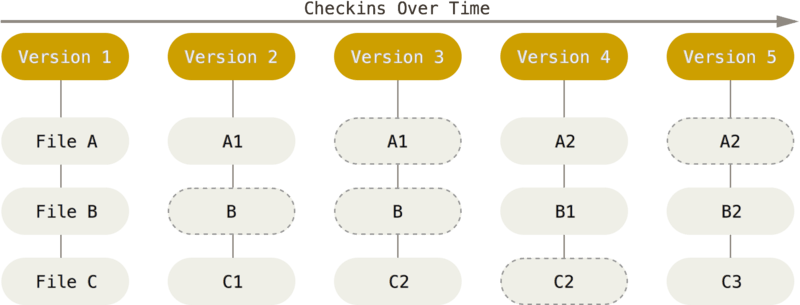
\includegraphics[width=.8\textwidth]{imgs/snapshots-git.png}
    
        \end{center}
    
    \end{block}
    

\end{frame}

\begin{frame}
    \frametitle{Git and GitHub}
    \framesubtitle{Getting started with Git}
    \addtocounter{nframe}{1}
    
    \textbf{Git has three main states that your files can reside in}

    \begin{block}{GIT DVCS}
       \begin{itemize}
           \item committed
           \item modified 
           \item staged
       \end{itemize}
    
    \end{block}

\end{frame}

\begin{frame}
    \frametitle{Git and GitHub}
    \framesubtitle{Getting started with Git}
    \addtocounter{nframe}{1}
    
    \begin{block}{GIT Areas}
        \begin{center}

            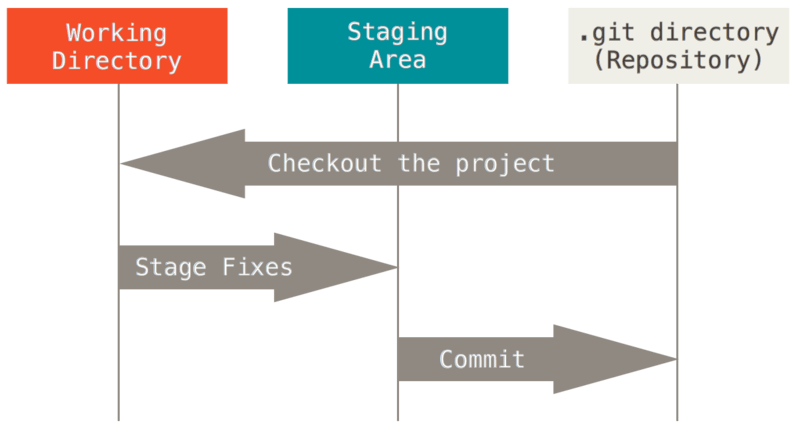
\includegraphics[width=.9\textwidth]{imgs/git-areas.png}
    
        \end{center}
    
    \end{block}
    

\end{frame}

\begin{frame}
    \frametitle{Git and GitHub}
    \framesubtitle{Getting started with Git}
    \addtocounter{nframe}{1}
    
    \textbf{Git has three main states that your files can reside in}

    \begin{block}{GIT local workflow}
       \begin{itemize}
           \item modify files in your working tree
           \item stage just those changes you want to be part of your next commit 
           \item do a commit which stores that snapshot permanently to your git directory
       \end{itemize}
    
    \end{block}

\end{frame}
